\section{What is optimisation?}


Discipline of applied mathematics. The idea is to search values for \alert{variables}\hspace{-1pt} in a given \alert{domain} that\hspace{-1pt} maximise/minimise\hspace{-1pt} \alert{function values}. 

Can be achieved by 
\begin{itemize}
	\item Analysing properties of functions \hspace{-1pt}/ extreme points or
	\item Applying numerical methods 
\end{itemize}


Optimisation has important applications in fields such as 

\begin{itemize}
	\item {\bf operations research (OR)};
	\item economics;
	\item statistics; 
	\item machine learning and artificial intelligence.
\end{itemize}



\subsection{Mathematical programming and optimisation}


In this course, optimisation is viewed as the core element of \alert{mathematical programming}.

Math. programming is a central OR modelling paradigm:
\begin{itemize}
	\item {\bf variables} $\rightarrow$ decisions: business decisions, parameter definitions, settings, geometries, ...;
	\item {\bf domain} $\rightarrow$ constraints: logic, design, engineering, ...;
	\item {\bf function} $\rightarrow$ objective function: measurement of (decision) quality. 
\end{itemize}

However, math. programming has many applications in fields other than OR, \alert{which causes some confusion}; 


\subsection{Types of mathematical optimisation models}

The \alert{simpler are the assumptions} which define a type of problems, the better are the \alert{methods to solve such problems}.

Some useful notation:

\begin{itemize}
	\item $x \in \reals^n$: vector of (decision) variables $x_j$, $j = 1,\dots, n$;
	\item $f:\reals^n \rightarrow \reals \cup \braces{\pm \infty}$: objective function;
	\item $X \subseteq \reals^n$: ground set (physical constraints);
	\item $g_i, h_i : \reals^n \rightarrow \reals$: constraint functions; 
	\item $g_i(x) \leq 0$ for $i = 1, \dots, m$: inequality constraints;
	\item $h_i(x) = 0$ for $i = 1, \dots, l$: equality constraints;
\end{itemize}


\begin{frame}{Types of programming}

Our goal will be to solve variations of the general problem $P$:
%
\begin{align*}
	(P) :~ \minf \ & f(x) \\
	\stf & g_i(x) \leq 0, i = 1, \dots, m\\
	& h_i(x) = 0, i = 1, \dots, l \\
	& x \in X.
\end{align*}
%

\begin{itemize}
	\item {\bf Linear programming (LP):} \alert{linear} $f(x) := c^\top x$ with $c \in \reals^n$; constraint functions $g_i(x)$ and $h_i(x)$ are \alert{affine} ($a_i^\top x - b_i$, with $a_i \in \reals^n$, $b \in \reals$); $X = \braces{ x \in \reals^n : x_j \geq 0, j =1,\dots,n}$.  
	\item {\bf (Mixed-)integer programming ((M)IP):} LP where (some of the) variables are \alert{binary (or integer)}. $X \subseteq \reals^k \times \braces{0,1}^{n-k}$ 
	\item {\bf Nonlinear programming (NLP):} some (or all) of the functions $f, g_i$ or $h_i$ are \alert{nonlinear};
	\item {\bf Mixed-integer\hspace{-1pt} nonlinear\hspace{-2pt} programming\hspace{-2pt} (MINLP):}\hspace{-1pt} {\small MIP\hspace{-3pt} +\hspace{-3pt} NLP.} 
\end{itemize}


\section{Linear programming applications}

\subsection{Resource allocation}


Most linear programming (LP) problems, can be interpreted as a \alert{resource allocation} problem. 


{\bf Problem statement:} define \alert{optimal plan} that maximises return/ minimise costs and \alert{satisfy rules}. Let

\begin{itemize}
	\item {\small $I = \braces{1, \dots, i, \dots, M}$}  - set of resources; 
	\item {\small $J = \braces{1, \dots, j, \dots, N}$} - set of products;
	\item $c_j$ - return per unit of product $j\in J$;
	\item $a_{ij}$ - resource $i\in I$ requirement for making product $j\in\hspace{-1pt} J$ ;
	\item $b_i$ - availability of resource $i\in I$; 
	\item $x_j$ - total production of $j \in J$.
\end{itemize}


{\bf Objective function:} measures the \emph{quality} of a production plan.
\begin{equation*}
	\maxi \sum_{j \in J}c_jx_j \Rightarrow c^\top x,
\end{equation*}
where $c = [c_1, \dots, c_{N}]^\top$ \hspace{-4pt} and $x = [x_1, \dots, x_{N}]^\top$ \hspace{-4pt} are $n$-sized vectors.


{\bf Constraints:} states the conditions for a plan to be \alert{valid}.
\begin{equation*}
	\st \sum_{j \in J} a_{ij}x_j \leq b_i, \forall i \in I	\Rightarrow	Ax \leq b,
\end{equation*}
where $a_{ij}$ are the components of the $M \times N$ matrix $A$ and $b = [b_1,\dots, b_M]^\top$. 

We also must require that $x_i \geq 0, \forall i \in I$.                                                                                                         


A paint factory produces \alert{exterior} and \alert{interior paint} from raw materials \alert{M1} and \alert{M2}. The \alert{maximum demand} for interior paint is 2 tons/day. Moreover, the amount of interior paint produced \alert{cannot exceed} that of exterior paint by more than 1 ton/day. 

\alert{Goal:} determine optimal paint production.
%

\begin{table}
	\begin{tabular}{rccc} \hline
	&\multicolumn{2}{c}{material (ton)/paint (ton)}\\ \hline
	& ext. paint & int. paint & daily availability (ton)\\ \hline
	material M1 & 6 & 4 & 24\\
	material M2 & 1 & 2 & 6\\ \hline
	profit (\$1000 /ton) & 5 & 4\\ \hline
	\end{tabular}
	\caption{Paint shop problem data} 
\end{table}


The complete model is:
%
\begin{flalign}
	\maxi z = \ &5x_1 + 4x_2 \label{eq:constM1}\\
	\st &6x_1 + 4x_2 \leq 24 \label{eq:constM2}\\
	&x_1 + 2x_2 \leq 6 \\
	&x_2 - x_1 \leq  1 \\
	&x_2 \leq 2 \\
	&x_1, x_2 \geq 0
\end{flalign}
%

The model could be also \emph{compactly represented} as

\begin{flalign*}
	\maxi z = \ & c^\top x \\
	&Ax \leq b\\
	&x \geq 0
\end{flalign*}
$c = [5, 4]^\top$, $x = [x_1, x_2]^\top$, 
$A = \begin{bmatrix} 6 & 4 \\ 1 & 2 \\ -1 & 1 \\0 & 1 \end{bmatrix}$ and 
$b = [24, 6, 1, 2]^\top$}


{\bf Problem statement}:    
\begin{itemize}
	\item plan production and distribution;
	\item transportation cost proportional \lb to distance travelled;
	\item factories have a capacity limit;
	\item clients have known demands.
\end{itemize}

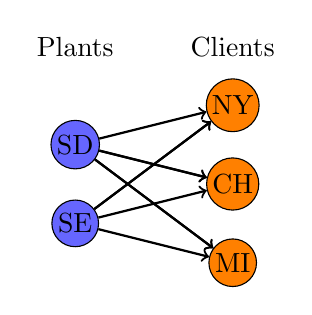
\begin{tikzpicture}[scale=1,
	node/.style={circle, fill=blue!60, draw, minimum size=1em, inner sep=1pt},
	node2/.style={circle, fill=orange, draw, minimum size=1em, inner sep=1pt}] 
    \node[above] at (0, 3.5) {Plants};                                                                                  
    \node[above] at (2, 3.5) {Clients};
    \node[node] (1) at (0, 1.5) {SE};
    \node[node] (2) at (0, 2.5) {SD};
    %\node[node] (3) at (0, 1) {3};
    %\node[node] (4) at (0, 0) {4};
    \node[node2] (3) at (2, 3) {NY};
    \node[node2] (4) at (2, 2) {CH};
    \node[node2] (5) at (2, 1) {MI};
    %\node[node2] (8) at (2, 0) {4};
   \onslide<1>
   \foreach \x in {1,...,2} {
       \foreach \y in {3,...,5} {
          \draw[->, thick] (\x) -- (\y);
          }} 
    \onslide<2>      
    \draw[->, thick] (1) -- (3);
    \draw[->, thick] (2) -- (4);
    \draw[->, thick] (2) -- (5);                            
\end{tikzpicture}                    



\begin{center}
\begin{table}
\begin{tabular}{r|ccc|c}
    & & {\it Clients} &\\\hline
    {\it Factory} & NY & Chicago & Miami & Capacity \\\hline
    Seattle & 2.5      & 1.7    & 1.8   & 350 \\
    San Diego & 3.5 & 1.8 & 1.4 & 600 \\\hline
    Demands & 325 & 300 & 275 & - \\\hline
\end{tabular}
\caption{Problem data: unit transportation costs, demands and capacities}
\end{table}
\end{center}



\subsection{Transportation problem}


Let $i \in I = \{\text{Seattle}, \text{San Diego}\}$ be the index set representing factories. Similarly, let $j \in J = \{\text{New York}, \text{Chicago}, \text{Miami}\}$.


Three key steps:

\begin{enumerate}
\item {\bf Determine what needs to be decided} ({\it decision variables})


$x_{ij}$ be the amount produced in factory $i$ and sent to client $j$.


\item {\bf How solutions are assessed} ({\it objective function})

Minimise total distribution cost:
%
$$ \mini z = 2.5x_{11} + 1.7x_{12} + 1.8x_{13} + 3.5x_{21} + 1.9x_{22} + 1.4x_{23},
$$
%

which can be more compactly expressed as 
%
$$\mini z = \sum_{i \in I}\sum_{j \in J}c_{ij}x_{ij}$$
where $c_{ij}$ is the unit transportation cost from $i$ to $j$.
%
\end{enumerate}


\begin{enumerate}
\setcounter{enumi}{2}
\item {\bf The requirements that must be satisfied} ({\it constraints})
%
\begin{align*}
&x_{11} + x_{12} + x_{13} \leq 350 \text{ (cap. lim. Seattle)}\\
&x_{21} + x_{22} + x_{23} \leq 600 \text{ (cap. lim San Diego)}\\
&x_{11} + x_{21} \geq 325 \text{ (dem. in New York)}\\
&x_{12} + x_{22} \geq 300 \text{ (dem. in Chicago)}\\
&x_{13} + x_{23} \geq 275 \text{ (dem. in Miami)}.
\end{align*}
%
These constraints can be expressed in the \emph{more compact form}
%
\begin{align*}
&\sum_{j \in J} x_{ij} \leq C_i, \forall i \\
&\sum_{i \in I} x_{ij} \geq D_j, \forall j,
\end{align*}

where $C_i$ is the production capacity of factory $i$ and $D_j$ is the demand of client $j$.
\end{enumerate}



Transportation problems

The complete model:
\begin{align*}
\minf z = \ &2.5x_{11} + 1.7x_{12} + 1.8x_{13} + 3.5x_{21} + 1.9x_{22} + 1.4x_{23} \\
\stf &x_{11} + x_{12} + x_{13} \leq 350, \ 
x_{21} + x_{22} + x_{23} \leq 600\\
&x_{11} + x_{21} \geq 325, \ x_{12} + x_{22} \geq 300, \ x_{13} + x_{23} \geq 275\\
&x_{11}, \dots, x_{23} \geq 0.
\end{align*}
%

Or, more compactly, in the so called \alert{algebraic (symbolic) form}
%
\begin{align*}
\mini z = \ &\sum_{i \in I}\sum_{j \in J}c_{ij}x_{ij}\\
\st & \sum_{j \in J} x_{ij} \leq C_i, \forall i\\
& \sum_{i \in I} x_{ij} \geq D_j, \forall j\\
&x_{ij} \geq 0, \forall i \in I, \forall j \in J.
\end{align*}

\end{frame}


\subsection{Production planning (lot-sizing)}


\begin{frame}{Production planning (lot sizing) problems}

      {\bf Problem statement}:    
      \begin{itemize}
      	\item plan \alert{production} ($p$) and \alert{storage} ($s$);
      	\item multiple periods with \alert{known demand} ($D$);
      	\item stock due to, e.g., different production costs ($C$) per period; 
      	\item stock can be \alert{held between periods}, for holding cost ($H$).
      \end{itemize}
	 
	 \vspace{6pt}
	 \centering
	 \pause
     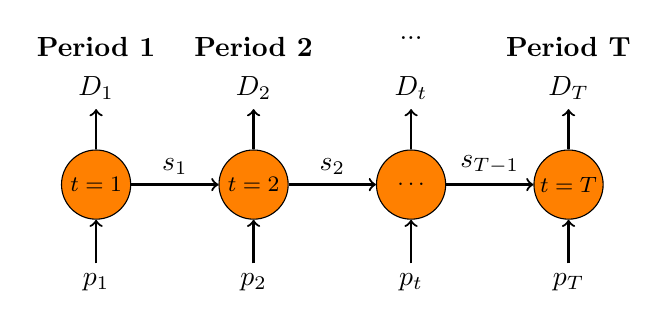
\begin{tikzpicture}[scale=1,
      node/.style={circle, fill=orange, draw, minimum size=2.5em, inner sep=1pt, font = \footnotesize}] 
%            	\draw (0,0) grid (6, 2) {};
            \node[below] at (0, 3) {\bf Period 1};                                                                                  
            \node[below] at (2, 3) {\bf Period 2};
            \node[below] at (4, 3) {...};
      	    \node[below] at (6, 3) {\bf Period T};
      	    \node[below] (11) at (0, 0) {$p_1$};                                                                                  
            \node[below] (21) at (2, 0) {$p_2$};
            \node[below] (31) at (4, 0) {$p_t$};
      	    \node[below] (41) at (6, 0) {$p_T$};
      	    \node[below] (12) at (0, 2.5) {$D_1$};                                                                                  
            \node[below] (22) at (2, 2.5) {$D_2$};
            \node[below] (32) at (4, 2.5) {$D_t$};
      	    \node[below] (42) at (6, 2.5) {$D_T$};	    
            \node[node] (1) at (0, 1) {$t=1$};
            \node[node] (2) at (2, 1) {$t=2$};
            \node[node] (3) at (4, 1) {$\dots$};
            \node[node] (4) at (6, 1) {$t=T$};
%           \foreach \x in {1,...,2} {
%               \foreach \y in {3,...,5} {
%                  \draw[->, thick] (\x) -- (\y);
%                  }} 
            \draw[->, thick] (1) -- node[above] {$s_1$} (2);
            \draw[->, thick] (2) -- node[above] {$s_2$} (3) ;
            \draw[->, thick] (3) -- node[above] {$s_{T-1}$}(4);
            \draw[->, thick] (11) -- (1);
            \draw[->, thick] (21) -- (2);
            \draw[->, thick] (31) -- (3);
            \draw[->, thick] (41) -- (4);   
            \draw[->, thick] (1) -- (12);
            \draw[->, thick] (2) -- (22);
            \draw[->, thick] (3) -- (32);
            \draw[->, thick] (4) -- (42);                                     
      \end{tikzpicture}                    
 
\end{frame}


\begin{frame}{Production planning (lot sizing) problems}

	Let
    \vspace{-6pt}
	\begin{itemize}
		\item $t \in \braces{1,\dots, T}$ -- set of time periods (e.g., months or days)
		\item $p_t$ -- amount \alert{produced} in period $t$
		\item $s_t$ -- amount \alert{stored} in period $t$, available for use in period $t+1$
		\item $P_t$, $H$ -- production/ holding costs  	
	\end{itemize}

	\pause
	The production planning problem can be stated as:
	%
	\begin{flalign*}
		\mini & \sum_{t \in T} \left[C_t p_t + H s_t\right] \\
		\st & p_t + s_{t-1} = D_t + s_t,  ~\forall t \in T \\
		& p_t, h_t \geq 0,  ~\forall t \in T .	
	\end{flalign*}
	%
	\pause
	{\bf Remarks:}
	\vspace{-6pt}
	\begin{itemize}
		\item Must carefully consider \alert{boundary conditions} ($t = T$; $t=0$)
		\item Production capacity constraints and uncertain demand can also call for inventory.	
	\end{itemize}
\end{frame}


\section{The geometry of LPs - graphical method} 



\begin{frame}{The geometry of linear problems}

	Consider the resource allocation model from before:
	\begin{columns}
		\column{0.45\textwidth}
		\begin{flalign*}
		\maxi z = \ &5x_1 + 4x_2 \\
		\st &6x_1 + 4x_2 \leq 24 \\
		&x_1 + 2x_2 \leq 6 \\
		&x_2 - x_1 \leq  1 \\
		&x_2 \leq 2 \\
		&x_1, x_2 \geq 0
		\end{flalign*}
		\column{0.45\textwidth}	
		\begin{flalign*}
			\maxi & z = c^\top	x \\
			\st & Ax \leq b \\
			& x \geq 0,
		\end{flalign*}
		where $A$ is an $m \times n$ matrix, and $b$, $c$, and $x$ have suitable dimensions.
	\end{columns}
	
	\pause
	\vspace{12pt}
	Let $a_i$ be one of the $m$ rows of $A$. Notice the following:
		\begin{itemize}
			\item Each constraint $a_i^\top x \leq b_i$ defines a \alert{closed half-space}, with boundary defined by a \alert{hyperplane} $a_i^\top x= b_i$.
			\item The \alert{feasible set} is the intersection of all closed half-spaces.	
		\end{itemize}

		
\end{frame}



\begin{frame}{Production planning - graphical representation}

\center
\includegraphics[scale=0.99]{Figures/ex2_c1.pdf}

\end{frame}

\begin{frame}{Production planning - graphical representation}

\center
\includegraphics[scale=0.99]{Figures/ex2_c2.pdf}

\end{frame}


\begin{frame}{Production planning - graphical representation}

\center
\includegraphics[scale=0.99]{Figures/ex2_c3.pdf}

\end{frame}


\begin{frame}{Production planning - graphical representation}

\center
\includegraphics[scale=0.99]{Figures/ex2_c4.pdf}

\end{frame}


\begin{frame}{Production planning - graphical representation}

\center
\includegraphics[scale=0.99]{Figures/ex2_c5.pdf}

\end{frame}


\begin{frame}{Production planning - graphical representation}

\center
\includegraphics[scale=0.99]{Figures/ex2_complete.pdf}

\end{frame}


\begin{frame}{LP geometry}

Some important concepts:
\begin{columns}

\column{0.45\textwidth}
\begin{enumerate}[<+->]
\item \alert{Active constraints:} resources (requirements) fully depleted (minimally satisfied).

{\bf Ex.:} {\color{blue}$6x_1 + 4x_2 \leq 24$} and \alert{$x_1 + 2x_2 \leq 6$}.   

\item \alert{Inactive constraints:} resources (requirements) not fully depleted (over satisfied).

{\bf Ex.:} {\color{green}$-x_1 + x_2 \leq 1$}.
\end{enumerate}

\column{0.55\textwidth}
\hspace{-0.25cm}
\includegraphics[width=\linewidth]{Figures/ex2_complete.pdf}

\end{columns}
\vspace{-6pt}
\onslide<3->{
Notice how making $n = 2$ constraints active out of $m = 4$ constraints \alert{forms a vertex}. However, not all vertices are feasible. 
}

\end{frame}


\begin{frame}{More on LP geometry}

The \alert{gradient} $\nabla z=[\frac{\partial z}{\partial x_1},\frac{\partial z}{\partial x_2}]^\top=[5,4]^\top$ indicates the direction in which $z$ increases; when minimising, we move towards $-\nabla z$. 
\vspace{-6pt}
\begin{center}
\includegraphics[scale = 0.7]{Figures/ex2_complete.pdf}
\end{center}
\vspace{-15pt}
Thus, in general, the solution is unique and \alert{lies on a vertex}. This turns the space of candidate solutions to be investigated \alert{finite}.

\end{frame}


\begin{frame}{More on LP geometry}

Since the feasible region is a \alert{polyhedral set} and the search direction is constant, we have that:
\begin{enumerate}[<+->]
	\item The number of candidate optimal solutions is (typically) \alert{finite}.
	\item A candidate optimal solution is (typically) a \alert{vertex}.
	\item The number of candidates increases \alert{exponentially} with the number of constraints and variables	
\end{enumerate}

\onslide<+->
The \alert{simplex method} exploits the above by: 
\begin{enumerate}[<+->]
	\item If the variable space is $\reals^n$, then \alert{$n$ active constraints form a vertex}.
	\item \alert{Heuristically} search for solutions by selecting $n$ constraints to be active from the $m$ constraints available. 
	\item Repeats until no improvement can be observed. When such, the \alert{geometry} of the problem guarantees \alert{(global) optimality}. 	
\end{enumerate}


 
 


\end{frame}


%\begin{frame}{Portfolio optimization}
%
%{\bf Problem statement.} Plan portfolio of assets to minimise exposition to risk (Markowitz). Let
%\begin{columns}
%\column{0.5\textwidth}
%\begin{itemize}
%\item {\small $J = \braces{1, \dots, j, \dots, N}$} assets;
%\item $\mu_j$ - expected relative return of asset $j \in J$;
%\item $\Sigma$ - covariance matrix;
%\item $\epsilon$ - minimum expected return;
%\item $x_j$ - position of asset $j \in J$
%\end{itemize}
%
%\column{0.4\textwidth}
%\pause
%\begin{align*}
%\mini \ &  x^\top\Sigma x  \\
%\st & \mu^\top x  \geq \epsilon\\
%& 0 \leq x_j \leq 1, \forall j \in J
%\end{align*} 
%\end{columns}
%\vfill
%\pause
%{\bf Remarks:} 
%\begin{itemize}
%\item The term $x^\top\Sigma x$ measures \alert{exposition to risk}. It is credited to Harry Markowitz (1952).
%\item Another important class: \alert{quadratic programming} (nonlinear).
%\end{itemize}
%
%\end{frame}
%
%
%\subsection{The pooling problem: refinery operations planning}
%
%
%\begin{frame}{Refinery Operations Planning Problem}
%
%\begin{columns}
%\column{0.6\textwidth}
%{\bf Oil refinery operational planning}
%\begin{itemize}
%	%% Juho: Small suggestion
%	\item Goal is to maximize profit;
%	%\item Seeks to maximize profit;
%	\item Several possible configurations;
%	\item \alert{Product property specifications} must be met;
%   \end{itemize}
%\column{0.4\textwidth}
%\begin{figure}
%\includegraphics[width=\linewidth]{figures/Refinery.png}
%\end{figure}
%\end{columns}
%\pause
%\begin{columns}
%\column{0.6\textwidth}
%{\bf Model characteristics:}
%	\begin{itemize}
%	\item \alert{Bilinear (nonconvex) and mixed-integer};
%	\item Large number of flows;
%	\item Several nonlinear constraints.
%    \end{itemize}
%\column{0.4\textwidth}
%\begin{figure}
%\includegraphics[width=\linewidth]{figures/RefinerySchema.png}
%\end{figure}
%\end{columns}
%
%\end{frame}
%
%
%\begin{frame}{Refinery Operations Planning Problem}
%
%\begin{columns}
%\column{0.65\textwidth}
%% First column
%
%{\bf Objective:} maximize profit
%
%{\bf Variables:}
%	\begin{itemize}
%	\item Stream Flows {\footnotesize(crude, intermediate and final products)};
%    \item Storage;
%    \item Stream properties.
%    \end{itemize}
%{\bf Constraints}
%	\begin{itemize}
%	\item Mass balance;
%    \item Market features (supply and demand);
%    \item Unit capacities;
%    \item Stream property limits;
%    \item \alert{Calculation of mix properties (nonlinear)}.
%    \end{itemize}
%\column{0.4\textwidth}
%% Second column
%\begin{figure}
%\includegraphics[width=\linewidth]{figures/Refinery.png}
%\end{figure}
%\begin{figure}
%\includegraphics[width=\linewidth]{figures/RefinerySchema.png}
%\end{figure}
%\end{columns}
%\end{frame}
%
%
%\begin{frame}{Refinery Operations Planning Problem}
%
%%% Juho: I think this is more precise.
%%The challenging aspect pertains to the quality of mixes. Let:
%The challenging aspect is how to model the calculation of product properties in a \alert{mix}. Let:
%%\vspace{-18pt}
%\begin{itemize}
% \item $x_p$ be the volume of product $p \in P$ and
% \item $q_p$ the value of a given chemical property (sulphur content, octane content, viscosity...).
%\end{itemize}
%%
%In a given mix, mass and property balances are calculated as:
%
%\begin{columns}
%\column{0.5\textwidth}
%\centering
%\includegraphics[scale=0.6]{Figures/Mixer.pdf}
%%
%\column{0.5\textwidth}
%%
%\begin{align*}
%& x_A = x_B + x_C \\ 
%& q_A = \frac{q_Bx_B + q_Cx_C}{x_A}  
%\end{align*}
%%
%\end{columns}
%\pause
%{\bf Remarks:} 
%\begin{itemize}
%\item More complex mixes (such as volumetric balances) might need to be considered.
%\item These are \alert{bilinear programming} problems (nonlinear).
%\end{itemize}
%\end{frame}
%
%
%\subsection{Robust optimisation}
%
%
%\begin{frame}{Robust optimisation}
%
%Is a subarea of mathematical programming concerned with \alert{uncertainty in the input data}.
%
%It's a risk-averse perspective that seeks \alert{protection against variability}.
%
%\pause
%%% Juho
%Consider the resource allocation problem under uncertainty:
%%Consider the resource allocation under uncertainty problem:
%%
%\begin{align*}
%\maxi \ &  c^\top x \\
%\st & \tilde{a}_{i}^\top x \leq b_i, \forall i \in I\\
%& x_j \geq 0, \forall j \in J
%\end{align*}
%
%%% Juho
%where $\tilde{a}_{i}$ is a \alert{random variable}.
%%We consider that $\tilde{a}_{i}$ is a \alert{random variable}.
%
%\end{frame}
%
%
%\begin{frame}{Robust optimisation}
%
%\includegraphics[width = 1\textwidth]{Figures/data_no_ellipsoid.pdf}
%
%\end{frame}
%
%
%\begin{frame}{Robust optimisation}
%
%%% Juho
%Assume that,\hspace{-1pt} for\hspace{-1pt} any\hspace{-1pt} $i \in I$, $\tilde{a}_{i} \in \epsilon_i = \braces{\overline{a}_i + P_iu : ||u||_2 \leq \Gamma_i}$, where 
%\vspace{-18pt}
%%Assume that, for a given $i \in I$, $\tilde{a}_{i} \in \epsilon_i = \braces{\overline{a_i} + P_iu : ||u||_s \leq \Gamma_i}$, where 
%
%\begin{itemize}
%\item $\overline{a}_{i}$ is the nominal (average) value; 
%%% Juho: I added the \epsilon here
%\item $P_i$ is the characteristic matrix of the ellipsoid $\epsilon$;
%\item $\Gamma_i$ is risk-aversion control parameter.
%\end{itemize}
%%
%\pause
%Then, the \alert{robust counterpart} can be stated as
%%
%\begin{align*}
%\maxi \ &  c^\top x \\
%\st & \max_{a_{i} \in \epsilon_i}\braces{a_i^\top x} \leq b_i, \forall i \in I\\
%& x_j \geq 0, \forall j \in J.
%\end{align*}
%\vspace{-6pt}
%%
%\pause
%Notice that 
%$$
%\max_{a_{i} \in \epsilon_i}\braces{a_i^\top x} = \overline{a}_i^\top x + \max_u\braces{u^\top P_i x : ||u||_2 \leq \Gamma_i} = \overline{a}_i^\top x + \Gamma_i||P_i x||_2 
%$$
%
%\end{frame}
%
%
%\begin{frame}{Robust optimisation}
%%
%The \alert{robust counterpart} can be equivalently stated as:
%\begin{align*}
%\maxi \ &  c^\top x \\
%\st & \overline{a}_i^\top x + \Gamma_i||P_i x||_2 \leq b_i, \forall i \in I\\
%& x_j \geq 0, \forall j \in J.
%\end{align*}
%%
%{\bf Remarks:}
%\begin{itemize}
%\item In case data is available, $P_i$ can be obtained from the \alert{empirical covariance matrix};
%%% Juho: A minor suggestion
%\item Values of $\Gamma_i$ can be drawn, for example, from a Chi-squared distribution. $\Gamma_i$ is sometimes called the \alert{budget of uncertainty}.
%%\item $\Gamma_i$ can be set according to, for example, Chi-squared distributions. In some contexts, it is called the \alert{budget of uncertainty}.
%\end{itemize}
%
%\end{frame}
%
%
%\begin{frame}{Robust optimisation}
%
%\includegraphics[width = 1\textwidth]{Figures/data_with_ellipsoid.pdf}
%
%\end{frame}
%
%
%\subsection{Classification: support vector machines}
%
%
%\begin{frame}{Classification}
%
%Suppose we are given some data $D \subset \reals^n$ that can be \alert{separated} into two sets in $\reals^n$: $I^- = \braces{x_1,\dots, x_N}$ and $I^+ = \braces{x_1,\dots,x_M}$. 
%
%Each element in $D$ is an \alert{observation} of a given set of \alert{features}; belonging to either $I^-$ or $I^+$ defines a \alert{classification}.
%
%\pause
%Our task is to select a function $f:\reals^n \rightarrow \reals$ from a given family of functions such that
%$$
%f(x_i) < 0, \ \forall x_i \in I^- \text{ and } f(x_i) > 0, \ \forall x_i \in I^+.
%$$ 
%Typically, $f$ is selected as a \alert{linear classifier}, \ie, $f(x_i) = a^\top x_i - b$. 
%
%Of course, there is always the possibility of \alert{misclassification} and, therefore, we want to determine the \alert{best} possible classifier.
%
%\end{frame}
%
%
%\begin{frame}{Classification}
%
%\centering
%\includegraphics[width = \textwidth]{Figures/classes_with_classifier.pdf}
%
%\end{frame}
%
%
%\begin{frame}{Classification}
%
%Let us define the following \alert{error measures}:
%{\small
%\begin{align*}
%& e^-(x_i \in I^-; a, b) := \begin{cases} 0, \text{ if } a^\top x_i - b \leq 0, \\
%                                a^\top x_i - b, \text{ if } a^\top x_i - b > 0.
%                   \end{cases} \\
%& e^+(x_i \in I^+; a, b) := \begin{cases} 0, \text{ if } a^\top x_i - b \geq 0, \\
%                                b -  a^\top x_i, \text{ if } a^\top x_i - b < 0.
%                   \end{cases}                   
%\end{align*}}% 
%\pause
%Using \alert{slack variables} $u_i$, $i = 1,\dots,M$, and $v_i$, $i = 1,\dots,N$, to represent $e^X$ and $e^Y$, the optimal classifier is obtained from:
%{\small
%\begin{align*}
%(LC) ~:~ \mini \ & \sum_{i=1}^M u_i + \sum_{i=1}^N v_i \\
%\st & a^\top x_i - b - u_i \leq 0, i = 1,\dots,M \\
%& a^\top x_i - b + v_i \geq 0, i = 1,\dots,N \\
%& ||a||_2 = 1\\
%&u_i \geq 0, i = 1,\dots,M; v_i \geq 0, i = 1,\dots,N; a \in \reals^n, b \in \reals.
%\end{align*}}
%%
%{\bf Remark:} notice that $||a||_2 = 1$ avoids $(a,b) = (0,0)$. 
%\end{frame}
%
%
%\begin{frame}{Classification}
%
%In practice, we can enforce a \alert{slab} $S = \braces{-1 \leq a^\top x_i- b \leq 1}$ as a buffer to trade off the \alert{robustness} of the classifier to outliers. 
%
%Accordingly, we redefine our error measures as follows. 
%%
%\begin{align*}
%& e^-(x_i \in I^-; a, b) := 
%    \begin{cases} 0, \text{ if } a^\top x_i - b \leq -1, \\
%        a^\top x_i - b, \text{ if } a^\top x_i - b > -1.
%    \end{cases} \\
%& e^+(x_i \in I^+; a, b) := 
%    \begin{cases} 0, \text{ if } a^\top x_i - b \geq 1, \\
%        b -  a^\top x_i, \text{ if } a^\top x_i - b < 1.
%    \end{cases}                   
%\end{align*}
%%
%\pause
%$e^-$ and $e^+$ include \alert{misclassifications} and \alert{correct classifications that lie within $S$}. The latter are know as \alert{support vectors}.
%
%The \alert{width of $S$ is given by $2/||a||_2$}, which is the distance between the hyperplanes $a^\top x_i - b = -1$ and $a^\top x_i - b = 1$.
%
%\end{frame}
%
%\begin{frame}{Classification}
%
%The robust version of $(LC)$ incorporating this buffer becomes   
%%
%\begin{align*}
%\mini \ & \sum_{i=1}^M u_i + \sum_{i=1}^N v_i + \gamma||a||_2^2\\
%\st & a^\top x_i - b - u_i \leq -1, \ i = 1,\dots,M \\
%& a^\top x_i - b + v_i \geq \p{-}1, \ i = 1,\dots,N \\
%&u_i \geq 0, i = 1,\dots,M; v_i \geq 0, i = 1,\dots, N; \\
%& a \in \reals^n, b \in \reals.
%\end{align*} 
%\pause
%{\bf Remarks:}
%\vspace{-6pt}
%\begin{itemize}
%\item The parameter $\gamma$ controls the \alert{trade-off} between the width of the slab $S$ and the number of observations within the slab.
%\item This quadratic programming problem is known in the machine learning literature as \alert{support vector machine}.
%\end{itemize}
%
%\end{frame}
%
%
%\begin{frame}{Classification}
%
%\centering
%\includegraphics[width = \textwidth]{Figures/classes_with_robust_classifier.pdf}
%
%\end{frame}
